\section{The number of cycles}\label{sec:cycles}

This section proves Theorem~\ref{thm:cycles}. The main step is Lemma~\ref{lem:through}.
Appendix~\ref{app:lean} names the Lean declaration for each step.

\subsection{The lower bound}

Entringer and Slater proved that $\psi(r)>2^{r-1}$ for $r\ge3$. Their examples are cubic: a cycle of
even length with all its long diagonals. These graphs give
$\psi(r)\ge2^{r-1}+r^{2}-3r+3$~\cite[Corollary~4]{ES}.

A simpler example suffices here. Let $j\ge2$. Take vertices $u_1,\dots,u_j$ and, for each $i$, two
further vertices $x_i$ and $y_i$ that are joined to $u_i$ and to $u_{i+1}$, with indices modulo $j$.
This is a ring of $j$ four-cycles: a chain like $N$ in Figure~\ref{fig:twoports}, closed up. It has
$3j$ vertices and $4j$ edges, so its rank is $j+1$. Its cycles are the $j$ four-cycles and the
$2^{j}$ cycles that pass through all the vertices $u_i$. So $\psi(r)\ge2^{r-1}+r-1$ for $r\ge3$.
The formal proof uses a closed chain of shortcuts from the construction of
Section~\ref{sec:upper} instead, which has rank $j+1$ and at least $2^{j}$ cycles.

\subsection{The upper bound}

In this subsection $G$ is a connected simple graph of rank $r$, and $k$ is an integer with
$1\le k\le r$.

\begin{lemma}[Independent edges]\label{lem:indep}
There is a set $D$ of $k$ edges of $G$ such that exactly $2^{r-k}$ even subgraphs of $G$ contain no
edge of $D$. Every edge of $D$ lies on a cycle of $G$.
\end{lemma}

\begin{proof}
Fix a spanning tree of $G$. Exactly $r$ edges of $G$ lie outside the tree. Let $D$ consist of $k$
of them. The graph $G-D$ contains the tree, so it is connected, and its rank is $r-k$. The even
subgraphs of $G$ that contain no edge of $D$ are the even subgraphs of $G-D$. So there are
$2^{r-k}$ of them. An edge of $D$ lies on a cycle, because the tree contains a path between its
ends.
\end{proof}

\paragraph{Chords and triangles.}
Let $e=uv$ be an edge of $D$. It lies on a cycle, so $v$ has a neighbour $w_e\ne u$. Fix such a
neighbour for each edge of $D$. If $u$ and $w_e$ are not adjacent in $G$, add the edge $uw_e$ and
call it a \emph{chord} (Figure~\ref{fig:chord}). Let $G^{+}$ be the graph that we get when we add
all chords, each of them once, and let $a\le k$ be the number of chords. The graph $G^{+}$ is simple
and connected, and it has the same vertices as $G$. So $\beta(G^{+})=r+a$.

For $e\in D$ let $T_e$ be the triangle of $G^{+}$ with the edges $uv$, $vw_e$ and $uw_e$, and let
$W$ be the union of these triangles. Then $W$ is a nonempty union of cycles of $G^{+}$, with at most
$3k$ edges and at most $k$ components. It contains every edge of $D$ and every chord. Every chord
$f$ lies on a triangle $T_f$ of $W$ whose other two edges are edges of $G$. If there are several
such triangles, fix one of them.

\begin{figure}[ht]
\centering
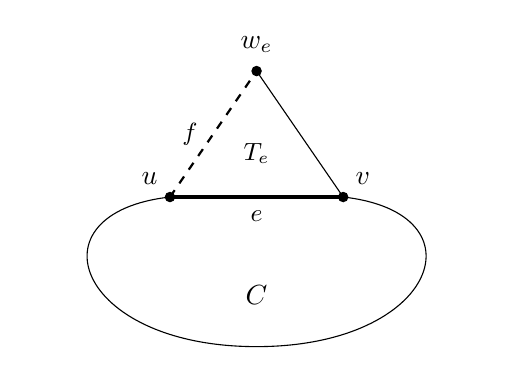
\begin{tikzpicture}
  \coordinate (u) at (0,0);
  \coordinate (v) at (2.2,0);
  \coordinate (w) at (1.1,1.6);
  \draw (v) .. controls (4.0,-0.2) and (3.4,-1.9) .. (1.1,-1.9)
            .. controls (-1.2,-1.9) and (-1.8,-0.2) .. (u);
  \draw[very thick] (u) -- node[below=1pt] {\small$e$} (v);
  \draw (v) -- (w);
  \draw[dashed,thick] (u) -- node[left=2pt] {\small$f$} (w);
  \foreach \p in {u,v,w} \fill (\p) circle (1.9pt);
  \node[above left=1pt] at (u) {$u$};
  \node[above right=1pt] at (v) {$v$};
  \node[above=3pt] at (w) {$w_e$};
  \node at (1.1,-1.25) {$C$};
  \node at (1.1,0.55) {\small$T_e$};
\end{tikzpicture}
\caption{An edge $e=uv$ of $D$, a second neighbour $w_e$ of $v$, and the chord $f=uw_e$ (dashed).
The chord is added if $u$ and $w_e$ are not adjacent in $G$. A cycle $C$ through $e$ and the even
subgraph $C+T_e$ have the same edges outside the triangle $T_e$.}
\label{fig:chord}
\end{figure}

\begin{lemma}[Cycles through $D$]\label{lem:through}
At most $p(G^{+},W)\,2^{r}$ cycles of $G$ contain an edge of $D$.
\end{lemma}

\begin{proof}
Let $F$ be the set of chords, so $|F|=a$. For a cycle $C$ of $G$ that contains an edge of $D$, and
for a set $S\subseteq F$, put
\[
  C_S=C+\sum_{f\in S}T_f .
\]
This is an even subgraph of $G^{+}$. We show two things.

\emph{The outside part of $C_S$ is a forest.} All triangles lie in $W$, so
$C_S\sm E(W)=C\sm E(W)$. The cycle $C$ contains an edge of $D$, and $D\subseteq E(W)$. So
$C\sm E(W)$ is a forest by Lemma~\ref{lem:count}(a).

\emph{The even subgraph $C_S$ determines the pair $(C,S)$.} The cycle $C$ contains no chord. The
triangle $T_f$ contains the chord $f$ and no other chord. So the set of chords in $C_S$ is $S$. Thus
$C_S$ determines $S$, and then it determines $C=C_S+\sum_{f\in S}T_f$.

Let $q$ be the number of cycles of $G$ that contain an edge of $D$. The sets $C_S$ are $q\,2^{a}$
distinct even subgraphs of $G^{+}$ whose outside part is a forest. By~\eqref{eq:count}, applied to
$G^{+}$ and $W$, there are exactly $p(G^{+},W)\,2^{r+a}$ such even subgraphs. Hence
$q\le p(G^{+},W)\,2^{r}$.
\end{proof}

\begin{proof}[Proof of Theorem~\ref{thm:cycles}]
Let $G$ be a graph of rank $r$, where $r$ is large. If $G$ is not connected, add a new vertex and
join it to one vertex of each component. The new edges are bridges, so the rank and the set of
cycles do not change. So we may assume that $G$ is connected.

Let $k$ be the least integer with $2^{k}>\log r$. Then $k\le\log\log r+1$, and $1\le k\le r$. Take
$D$ as in Lemma~\ref{lem:indep}, and take $G^{+}$ and $W$ as above. A cycle of $G$ avoids $D$ or
contains an edge of $D$. At most $2^{r-k}<2^{r}/\log r$ cycles avoid $D$, by
Lemma~\ref{lem:indep}. At most $p(G^{+},W)\,2^{r}$ cycles contain an edge of $D$, by
Lemma~\ref{lem:through}.

It remains to bound $p(G^{+},W)$. The graph $G^{+}$ is connected and simple, and its rank
$r^{+}=r+a$ is at least $r$. The subgraph $W$ is a nonempty union of cycles. It has at most
$3k\le\sqrt{r}\le\sqrt{r^{+}}$ edges and at most $k\le(\log r)/100\le(\log r^{+})/100$ components,
because $r$ is large. So Theorem~\ref{thm:forest} applies to $G^{+}$ and $W$, and
\[
  p(G^{+},W)\;\le\;\frac12+\frac{20}{\lgk3r^{+}}\;\le\;\frac12+\frac{20}{\lgk3r}.
\]
Altogether, the number of cycles of $G$ is at most
\[
  \Bigl(\frac12+\frac{20}{\lgk3r}+\frac1{\log r}\Bigr)2^{r}
  \;\le\;\Bigl(\frac12+\frac{21}{\lgk3r}\Bigr)2^{r},
\]
because $\lgk3r\le\log r$. Together with the lower bound, this gives $\psi(r)\sim2^{r-1}$.
\end{proof}

\begin{remark}\label{rem:chords}
The choice of $k$ is not delicate. The proof needs $2^{-k}\le1/\lgk3r$ for the cycles that avoid
$D$, and $100k\le\log r$ for the components of $W$.

The chords are the point of the proof. Without them one would take for $W$ a union of cycles of $G$
through the edges of $D$. Such cycles can be long, and Theorem~\ref{thm:forest} needs $W$ to be
small. To shorten them one would have to pass to a cubic multigraph and search for short cycles
there. The chords create the short cycles directly, and Lemma~\ref{lem:through} shows that they cost
nothing.
\end{remark}
